\documentclass[a4paper, 12pt]{report}
\usepackage[T2A]{fontenc} 
\usepackage[utf8]{inputenc}
\usepackage[english,russian]{babel} 
\usepackage{amsmath,amsfonts,amssymb,amsthm,mathtools}
\usepackage[left=2cm,right=2cm,top=2cm,bottom=2cm,bindingoffset=0cm]{geometry}
\usepackage{graphicx}
\usepackage[linesnumbered,boxed]{algorithm2e}
\usepackage{verbatim}

\newenvironment{Proof} 
{\par\noindent{$\blacklozenge$}}
{\hfill$\scriptstyle\boxtimes$} 

\newenvironment{example} 
{\par\noindent{\textsc{\textbf{Пример}.}}} 
{\hfill$\scriptstyle\Box$} 

\newtheorem*{theorem}{Теорема} 
\newtheorem*{corollary}{Следствие}
\newtheorem*{lemma}{Лемма}

\newcommand{\RNumb}[1]{\uppercase\expandafter{\romannumeral #1\relax}}
\newcommand{\Rm}{\mathbb{R}}
\newcommand{\Cm}{\mathbb{C}}
\newcommand{\I}{\mathbb{I}}
\newcommand{\N}{\mathbb{N}}
\newcommand{\Z}{\mathbb{Z}}
\newcommand{\Q}{\mathbb{Q}}

\title{\textbf{\Huge{Методы вычислений}}\\Лабораторная работа 3\\«Метод прогонки»\\Выполнила Николаева Ксения, 9 группа}
\date{} 

\begin{document}
    \maketitle

    \textbf{\Huge{Постановка задачи}}\\\\
    Написать и отладить программу (С++), реализующую метод прогонки для численного решения систем линейных алгебраических уравнений $Ay = f$ с трехдиагональной матрицей $A$ порядка $N + 1$\\
    Задача:\\
    Необходимо решить систему линейных алгебраических уравнений с трёхдиагональной матрицей $A$ порядка $n$. Матрица $A$ задаётся случайными значениями. Для решения необходимо реализовать метод прогонки.
\[
A =
\begin{pmatrix}
c_0 & b_0 & 0 & \cdots & 0 \\
a_1 & c_1 & b_1 & \cdots & 0 \\
0 & a_2 & c_2 & \cdots & 0 \\
\vdots & \vdots & \vdots & \ddots & \vdots \\
0 & 0 & 0 & a_{n} & c_{n}
\end{pmatrix}
\]

    где $a_i$, $b_i$, $c_i$ — элементы матрицы, заданные случайным образом.\\
    Вектор точного решения $y$ задать как:
    \[
   y = \begin{pmatrix}
   1 \\
   2 \\
   \vdots \\
   n + 1
   \end{pmatrix}
   \]
   где $m = 8$ — номер студента. Правую часть $f$ вычислить как $f_i = a_{i} \cdot y_{i - 1} + c_{i} \cdot y_{i} + b_{i} \cdot y_{i + 1}$.\\ 
   Вывести первые и последние 5 координат векторов $y$ и $ \tilde{y}$ (приближенное решение), а также относительную погрешность и время выполнения.\\
   

   \newpage
   \textbf{\Huge{Краткие теоретические сведения}}\\\\
   \textbf{Метод прогонки}, также известный как метод трёхдиагональной матрицы, является эффективным численным методом для решения систем линейных алгебраических уравнений, в которых матрица является трёхдиагональной. Такие матрицы имеют ненулевые элементы только на главной диагонали и двух соседних диагоналях.
\\\\
   \textbf{Формулы:}\\
   Метод прогонки состоит из двух основных этапов: прямого и обратного хода.
\\
1. Прямой ход:
   В этом этапе вычисляются коэффициенты $\alpha_i$ и $\beta_i$, которые помогают преобразовать систему уравнений в более простую форму. На этом этапе вычисляются значения, которые будут использоваться в обратном ходе.

   $$\alpha_{1} = -\frac{b_{0}}{c_{0}}$$
   $$\beta_{1} = -\frac{f_{0}}{c_{0}}$$
   $$\alpha_{i + 1} = -\frac{b_{i}}{c_{i} + a_{i} \alpha_{i}}$$
   $$\beta_{i + 1} = \frac{f_{i} - a_{i} \beta_{i}}{c_{i} + a_{i} \alpha_{i}}$$
   $$\beta_{n + 1} = \frac{f_{n} - a_{n} \beta_{n}}{c_{n} + a_{n} \alpha_{n}}$$
\\
2. Обратный ход:
   На этом этапе находятся значения вектора $\mathbf{y}$, используя ранее вычисленные коэффициенты.

   
   $$y_{n} = \beta_{n + 1}$$ 
   $$y_{i} = \alpha_{i + 1} y_{i+1} + \beta_{i + 1}$$

   \textbf{Погрешности в вычислениях}делятся на абсолютные и относительные\\
   $\bullet$ Абсолютная погрешность — это разность между истинным и вычисленным значениями\\
   $\bullet$ Относительная погрешность — отношение абсолютной погрешности к истинному значению:$$\delta =  \dfrac {||y - \tilde{y}||_{\infty}}{||y||_{\infty}}$$\\
   \\

   \newpage
   \textbf{\Huge{Листинг программы с комментариями}}\\\\
   \begin{verbatim}
#include <bits/stdc++.h>

using namespace std;

const int N = 1e3 + 1;
const int M = 1e3 + 9;
const int MOD = 1e9 + 7;
const long long INF = 1e18 + 9;

vector<long double> a, b, c;
vector<long double> f;
vector<long double> y;
vector<long double> y2;

int n;
int m = 8;

///Создание матрицы A
void createMatrix(int n) {
    srand(time(0));
    a.resize(n + 1, 0);
    b.resize(n + 1, 0);
    c.resize(n + 1, 0);

    for (int i = 1; i <= n; ++i) {
        a[i] = rand() % 201 - 100;
    }
    for (int i = 0; i < n; ++i) {
        b[i] = rand() % 201 - 100;
    }

    c[0] = abs (b[0]) + rand() % (m + 1) + m;
    c[n] = abs (a[n]) + rand() % (m + 1) + m;
    for (int i = 1; i < n; ++i) {
        c[i] = abs(a[i]) + abs(b[i]) + c[0] + rand() % (m + 1) + m;
    }
}

///Вычисление значений вектора f
void createF(int n) {
    f.resize(n + 1, 0);
    f[0] = c[0] * y[0] + b[0] * y[1];
    f[n] = a[n] * y[n - 1] + c[n] * y[n];
    for (int i = 1; i < n; ++i) {
        f[i] = a[i] * y[i - 1] + c[i] * y[i] + b[i] * y[i + 1];
    }
}

///Реализация метода прогонки
void TridiagonalMatrixAlgorithm (int n) {
    vector<long double> alpha(n + 2), beta(n + 2);

    /// Прямой ход прогонки
    alpha[1] = - b[0] / c[0];
    beta[1] = f[0] / c[0];
    for (int i = 1; i < n; ++i) {
        long double delta = c[i] + a[i] * alpha[i];
        alpha[i + 1] = - b[i] / delta;
        beta[i + 1] = (f[i] - a[i] * beta[i]) / delta;
    }
    beta[n + 1] = (f[n] - a[n] * beta[n]) / (c[n] + a[n] * alpha[n]);

    /// Обратный ход прогонки
    y2[n] = beta[n + 1];
    for (int i = n - 1; i >= 0; --i) {
        y2[i] = alpha[i + 1] * y2[i + 1] + beta[i + 1];
    }
}

///Вывод ответа для задачи
void printAnswer(int n) {
    cout << "Exact solution\n";
    for (int i = 0; i < 5; ++i) {
        cout << "y" << i << " = " << fixed << setprecision(20) << y[i] << '\n';
    }

    cout << "...\n";
    for (int i = n - 5; i <= n; ++i) {
        cout << "y" << i << " = " << fixed << setprecision(20) << y[i] << '\n';
    }
    cout << "---------------------\n";
    cout << "Approximate solution\n";
    for (int i = 0; i < 5; ++i) {
        cout << "~y" << i << " = " << fixed << setprecision(20) << y2[i] << '\n';
    }
    cout << "...\n";
    for (int i = n - 5; i <= n; ++i) {
        cout << "~y" << i  << " = " << fixed << setprecision(20) << y2[i] << '\n';
    }
    ///Подсчет относительной погрешности
    cout << "---------------------\n";
    cout << "Relative error\n";
    long double max_diff = 0, max_exact = 0;
    for (int i = 0; i <= n; ++i) {
        max_diff = max(max_diff, abs(y[i] - y2[i]));
        max_exact = max(max_exact, abs(y[i]));
    }
    long double relative_error = max_diff / max_exact;
    cout << scientific << setprecision(15) << relative_error << '\n';
}

int32_t main() {

    freopen("output.txt", "w", stdout);

    n = 999;
    y.resize(n + 1);
    y2.resize(n + 1);

    createMatrix(n);

    for (int i = 0; i <= n; ++i) {
        y[i] = i + 1;
    }
    createF(n);

    /// Решение системы через метод прогонки
    clock_t start = clock();
    TridiagonalMatrixAlgorithm(n);
    clock_t end = clock();
    long double elapsed_time = double(end - start) * 1000.0; /// Подсчет затраченного времени в миллисекундах
    printAnswer(n);
    cout << "Time Tridiagonal matrix algorithm: " << elapsed_time << " milliseconds\n";

    return 0;
}
   \end{verbatim}
   \newpage
   \textbf{\Huge{Результаты}}\\\\
   $\bullet$ Результат вычислительного экперимента для задачи\\
   \begin{center}
        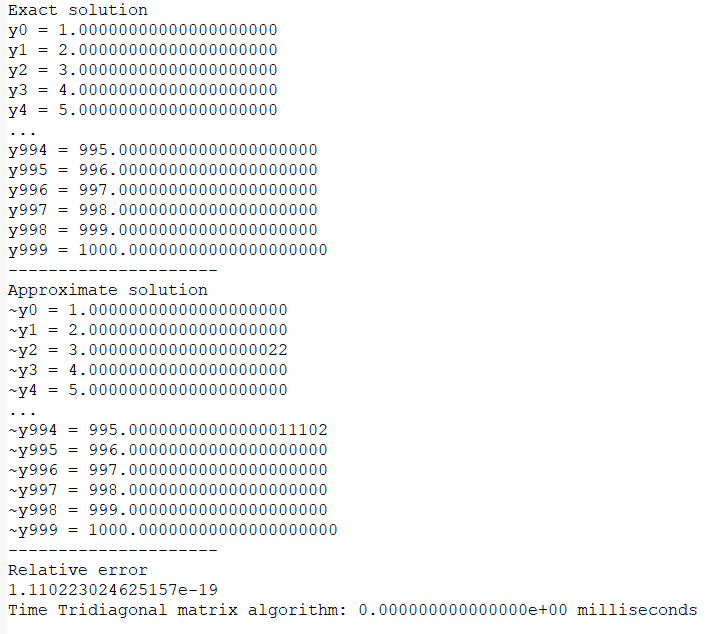
\includegraphics[scale = 0.7]{pic5.png}
   \end{center}
   

    \newpage
   \textbf{\Huge{Выводы}}\\\\
      В ходе выполнения лабораторной работы был реализован метод прогонки для решения систем линейных алгебраических уравнений с трёхдиагональными матрицами. Основные достижения и выводы работы следующие:\\

$\bullet$ Метод прогонки продемонстрировал высокую вычислительную эффективность, что позволило успешно решить систему уравнений размером $n = 999$ за время, не превышающее несколько миллисекунд. Это подтверждает его пригодность для задач, требующих быстрой обработки больших объемов данных.\\

$\bullet$ В ходе работы были получены как точные, так и приближенные решения системы. Проведен анализ относительной погрешности, который показал, что приближенное решение находится в допустимых пределах близости к точному решению, что свидетельствует о корректности реализации алгоритма.\\
   
\end{document}


